\documentclass[twocolumn]{article}
\usepackage{soul}
\usepackage{amsmath}
\usepackage[utf8]{inputenc}
\usepackage[left=2cm, right=2cm, top=50]{geometry}
\usepackage{multicol}
\setlength{\columnsep}{1cm}
\usepackage{graphicx}
\usepackage{subfigure}
\title{Straight Line}
\author{Diptasri Ghosh}
\date{EE21MTECH14004}

\begin{document}

\maketitle
\textbf{\textit{Abstract} - This document contains solution of plotting a straight line from the given equation.}\\
\begin{center}
\textbf{\ul{Problem}}\\
Vector-2, Example-5, Question No.-12
\end{center}

\textbf{Question 12. Trace the straight line whose equation is :}\\
\begin{equation}
5x - 7y -9 = 0
\end{equation}
\textbf{Solution :}\\
The given equation is,
\begin{equation}
5x - 7y -9 = 0
\end{equation}
We can write equation (2) as,
\begin{equation}
\begin{pmatrix}
5 & -7\\ 
\end{pmatrix} \textbf{x} = 9
\end{equation}
We can find different solutions of the equation (3) as , \\
Let 
\begin{equation}
\textbf{x} = \begin{pmatrix}
a \\ 
0\\
\end{pmatrix}
\end{equation}
Substituting in equation (3),
\begin{equation}
\begin{pmatrix}
5 & -7 \\ 
\end{pmatrix}\begin{pmatrix}
a\\ 
0\\
\end{pmatrix} = 9
\end{equation}
\begin{equation}
a = \frac{9}{5}
\end{equation}
Similarly we can consider,
\begin{equation}
\textbf{x} = \begin{pmatrix}
0\\ 
b\\
\end{pmatrix}
\end{equation}
Substituting in equation (3),
\begin{equation}
\begin{pmatrix}
5 & -7 \\ 
\end{pmatrix}\begin{pmatrix}
0\\ 
b\\
\end{pmatrix} = 9
\end{equation}
\begin{equation}
b = \frac{-9}{7}
\end{equation}
So, the intercepts of X and Y axes can be obtained as,
\begin{equation}
\textbf{A} = \begin{pmatrix}
\dfrac{9}{5}\\ 
0\\
\end{pmatrix} , 
\textbf{B} = \begin{pmatrix}
0\\
\dfrac{-9}{7}\\ 
\end{pmatrix}
\end{equation}

\begin{figure}[!ht]
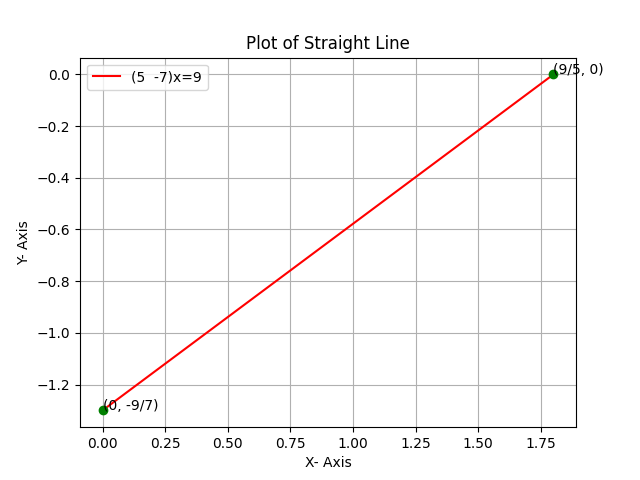
\includegraphics[width=1.1\columnwidth]{Figure_1.png}
\label{fig}
\end{figure}
\end{document}












